\documentclass[dvipdfmx,line_length=48zw,column_gap=2zw,number_of_lines=60,baselineskip=12pt]{jlreq}
\jlreqsetup{itemization_beforeafter_space=0pt}
\RenewBlockHeading{section}{1}{font={\normalsize\sffamily\gtfamily},indent=0pt,lines=1}
\RenewBlockHeading{subsection}{2}{font={\normalsize\sffamily\gtfamily},indent=0pt,lines=1}
\RenewBlockHeading{subsubsection}{3}{font={\normalsize\sffamily\gtfamily},indent=0pt,lines=1}
\pagestyle{empty}
%% ↑この上の部分は変更しない！
%% （LuaTeXを使う場合は \documentclass[dvipdfmx,... の dvipdfmx, を消す）
%%%%%%%%%%%%%%%%%%%%%%%%%%%

%% デフォルトでは詰め込むために見出しの行数は1行分となっています．
%% 見出しの前に1行分のスペースを入れるには以下を有効にしてください．
%% （section, subsection, subsubsection ごとに変更できます）
% \ModifyHeading{section}{before_lines=1}
% \ModifyHeading{subsection}{before_lines=1}
% \ModifyHeading{subsubsection}{before_lines=1}

%% 節タイトルが長くて，特定の見出しだけ2行分とりたい場合は，
%% 本文中で対象の見出しを以下のように書いてください．
%% もちろん，これをプリアンブルに書いて全ての見出しに適用することもできます．
% \ModifyHeading{section}{lines=2}
% \section{長い長い長い長い長い長い長い長い長い長い長い長い長い節}
% \ModifyHeading{section}{lines=1}

%%↓必要なパッケージを追加してください．
\usepackage[T1]{fontenc}
\usepackage{mathtools,amssymb}
\usepackage{newtxtext,newtxmath}
\usepackage[utf8]{inputenc} 	%波ダッシュ（〜）を表記できるようにする

\usepackage{muselabyoko} % ← muselabyoko.sty を読み込む

% \newcommand{\red}[1]{\textcolor{red}{#1}}
% \newcommand{\cut}[1]{\textcolor{red}{\sout{\textcolor{black}{#1}}}}
%%%%%%%%%%%%%%%%%%%%%%%%%%%
\begin{document}
\twocolumn[
    {\Large
            \begin{center}
                %%↓タイトルを入力してください
                % 卒業論文のタイトルを書く
持続音楽器におけるヴィブラート表現の整理と

教育的理解に向けた初期検討
                %%%%%%%%%%%%%%%%%%%%%%%%%%%
            \end{center}
        }
    \vspace{12pt}
    \begin{flushright}
        福知山公立大学情報学部　\input{../credit/author-name} \\
        指導教員　橋田光代
    \end{flushright}
    \vspace{1\Cvs}
]


%% ここから本文を書く
% !TEX root = _yoko.tex

% ==========================================
% プロジェクト予稿（1P）の本文
% ==========================================

\section{はじめに}

小型のハードウェアシンセサイザー等を複数用いたマシンライブは、ノブやフェーダー、ボタンによる微細かつ連続的なパラメータ制御や、時間的に安定したトリガー入力が可能であり、高い操作精度を有している。
一方で、操作が複雑になりやすく、曲中での即興的なアクセント付与が困難な場面が存在する。
また、入力インターフェースの小型化により演奏者の身体動作も小さくなり、身体動作と音響変化の関係性が視覚的に伝わりにくいという課題がある。
本研究では、身体動作と音響変化が直感的に対応する演奏体験の実現を目的とし、MediaPipe\cite{MediaPipe}を用いて演奏者の身体動作を直接MIDI制御へと変換するインタラクティブ演奏システムを提案する。
これにより、演奏行為そのものを視覚的・音響的表現として楽しめるものにし、電子楽器演奏における没入感の向上を目指す。

\section{システム概要}
本研究では、マシンライブにおける複雑な操作の容易化と、身体動作と音響変化の関係性が直感的に理解できる演奏体験の実現を目的として、ハンドジェスチャーによるMIDI制御システムを提案する。本システムは、容易な操作で多数の MIDI パラメータを制御できること、身体動作と音響変化の対応関係が視覚的・感覚的に理解しやすいこと、特別な機材を必要とせず容易に導入できることを設計方針としている。

システムは、MediaPipeにより手指の位置情報およびハンドサインをリアルタイムに検出し、その情報をMax上でMIDI制御信号へ変換する構成となっている。ユーザーは片手をカメラに映し、あらかじめ定義されたハンドジェスチャーを行うことで、シンセサイザー等のMIDI対応機器を直感的に操作することができる。

ジェスチャーは、単発的な信号を送信する「トリガージェスチャー」と、連続的に値を変化させる「コントロールジェスチャー」の 2 種類に分類される。
トリガージェスチャーには、複数のハンドサインやスワイプ動作を用い、ノートオン／オフや MIDI CC の出力を行う。
コントロールジェスチャーでは、カメラからの距離、手の開き具合、ノブを回す動作などを用いて、MIDI CC やピッチを連続的に制御する。

また、本システムでは、ジェスチャーと送信するMIDI情報の組み合わせを自由に設定できるパッチングシステムを構築し(\figref{fig:trigger_set})、これにより演奏者は自身の演奏スタイルや使用機材に応じた柔軟な設定を行うことが可能である。

\begin{figure}[tb]
	\centering
	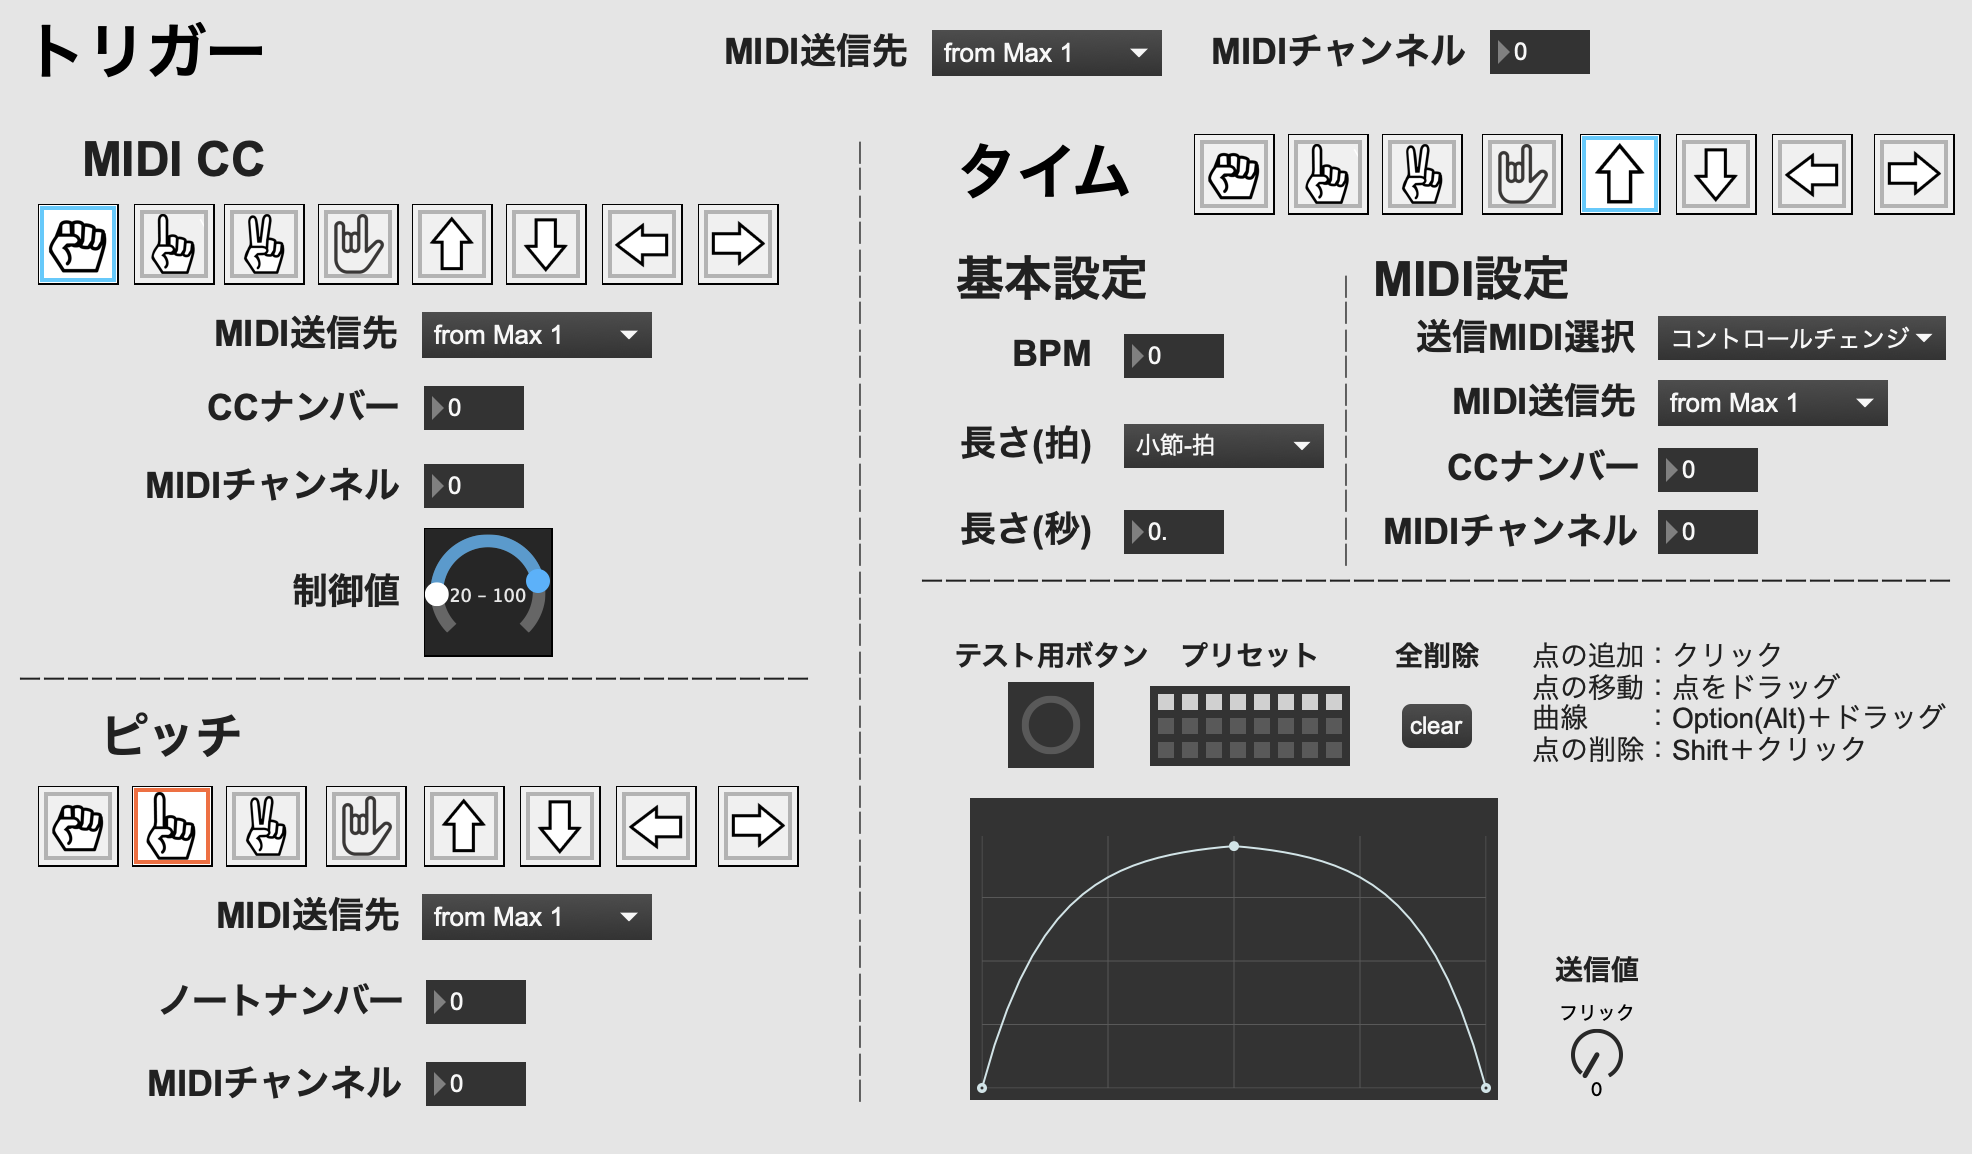
\includegraphics[width=\hsize]{../fig/trigger_set.png}
	\caption{トリガージェスチャー設定画面}
	\label{fig:trigger_set}
\end{figure}

これらの要素により、従来のマシンライブにおける操作の難しさを軽減するとともに、身体動作と音響変化が結びついた演奏が可能になる。

\section{実演と評価}
本システムの有効性を検証するため、研究室内にてゼミ生6名を対象に、構築したシステムを用いたマシンライブを実施した。
使用機材は小型シンセサイザー2台とPCであり、カメラにはPC内蔵カメラを用いた。

実演の結果、ユーザー視点では、片手のハンドジェスチャーによって複雑なMIDI操作を直感的に行えることが確認でき、位置を意識せずにパラメータ制御が可能であった。

また、観客視点からは、ジェスチャーと音響変化の関係性が理解しやすく、両者の一致による面白さや視覚的な没入感の向上が示唆された。

以上より、本システムはマシンライブにおける操作の容易化と視覚的没入感の増幅において有効であると考えられる。

\section{おわりに}
本研究では、マシンライブにおける演奏操作の容易化と即興的表現の拡張を目的として、ハンドジェスチャーによるMIDI制御演奏システムを提案・実装した。
MediaPipeを用いてジェスチャーを検出し、演奏動作と音響変化を柔軟に対応付けるMIDI出力機構を構築した。
実演を通じて、複雑な操作や即興的アクセント付けが容易になること、ならびに演奏動作と音響変化の一致による視覚的没入感の向上を確認した。
一方で、使用可能なジェスチャーの組み合わせに制限がある点が課題として残った。


% 参考文献
\bibliographystyle{../muselabunsrt} % bstファイルの名前
\bibliography{../onodera2025} % .bibファイルの名前（Zoteroからエクスポートして作る）

\end{document}
